\chapter[Características Fractales del Pan]{Validación: Características Fractales y Multifractales del Pan}

\section{Introducción}
Las imágenes generadas utilizando los métodos de los capítulos previos provocan la percepción de determinados materiales en escenas renderizadas.
Lamentablemente, el fenómeno de la percepción resulta difícil de cuantificar.
La computación gráfica ha apelado históricamente a métodos subjetivos de validación de resultados, debido a la complejidad de los fenómenos involucrados en los mecanismos de percepción humanos.
Uno de los métodos de validación clásicos consiste en realizar pruebas con personas, entreg\'andoles im\'agenes verdaderas y sint\'eticas, sin que los participantes del experimento sepan a cu\'al categor\'ia pertenece cada una, pidi\'endoles que clasifiquen las im\'agenes como verdaderas o sint\'eticas.
Si las im\'agenes sint\'eticas resultan ser clasificadas en un porcentaje adecuado como reales, se puede considerar al experimento como satisfactorio.
Si bien este método puede resultar interesante, se siguen requiriendo métodos automáticos y objetivos, ya que en este caso se sigue dependiendo de observadores subjetivos para evaluar la calidad de las imágenes.


Existen diversos criterios objetivos para evaluar la fidelidad de las im\'agenes resultantes.
Apelando a métodos matemáticos, podemos comparar imágenes por medio de extracci\'on de caracter\'isticas.
En el presente capítulo se comparan dimensiones fractales (\acrshort{DF}) y multifractales de determinadas caracter\'isticas de imágenes reales y sint\'eticas de cortes de panes.
Gracias a estas t\'ecnicas, podemos validar los resultados obtenidos en los cap\'itulos anteriores con una base matem\'atica s\'olida, m\'as all\'a de la validaci\'on visual realizada por personas, la cual se emplea tradicionalmente en computaci\'on gr\'afica.
Como aporte extra de la tesis, las características fractales y multifractales capturan detalles esenciales que pueden ser utilizados para la clasificación de las muestras, superando a otros clasificadores del estado del arte.


\section{Dimensiones fractales de imágenes de migas de pan}

Uno de los factores más importantes en la evaluación de la calidad de una muestra de pan está constituido por la estructura de su miga.
La observación de las burbujas de distintos cortes de pan nos revela una variación considerable en los tamaños y posiciones de las mismas, incluso si los cortes pertenecen a una única muestra de un tipo de pan.
Si bien estas estructuras parecen carecer de patrones repetitivos que caractericen al material, en este capítulo mostraremos que es posible, a nivel estadístico, caracterizar sus distribuciones de tamaños.

En \cite{Gonzales2008} se present\'o un trabajo de c\'alculo de distintas dimensiones mono-fractales sobre muestras de pan.
Las mismas son obtenidas a trav\'es de diversos algoritmos, diferentes a los utilizados en este trabajo.
En esta sección demostraremos que una única dimensión fractal, si bien constituye una aproximación adecuada en muchos casos, no resulta lo suficientemente descriptiva para capturar la riqueza de las distribuciones de burbujas en distintos tipos de panes.
Esto será demostrado realizando una caracterización y clasificación de distintas imágenes de muestras de pan.
Se utilizan las DFs de Korcak \cite{Mandelbrot1983} y la dimensi\'on Box \cite{Peitgen2004} sobre imágenes obtenidas por medios tradicionales (cámaras y escáneres), buscando caracterizar su estructura.


\subsection{Dimensi\'on Box}
La misma intenta simplificar el c\'alculo de la DF de Hausdorff, debido a que \'esta resulta muy dif\'icil de obtener \cite{Peitgen2004} (o imposible si el objeto no es estrictamente autosimilar).
Dada una imagen, se la subdividide en una grilla de dimensiones $M\times M$ donde el largo del lado de cada cuadrado formado es $\delta$. Si $N(\delta)$ representa el n\'umero de cuadrados que contienen al menos un p\'ixel resultado de una binarizaci\'on de la imagen (p\'ixel blanco) para ese $\delta$, la dimensi\'on Box $D_{b}$ queda definida como:\\

$$D_{b} = \displaystyle\lim_{\delta \to 0}{\frac{\log(N(\delta))}{\log (1/\delta)}}$$\\

En el algoritmo resultante se utiliza una imagen binarizada computada a partir de la original. Sobre la misma se seleccionan distintos $\delta$, realizando un conteo de cuadrados que contienen p\'ixeles blancos en cada caso (para evitar inestabilidad num\'erica, se utiliza un promedio de casos, estableciendo distintas posiciones de la grilla sobre la imagen). Finalmente se realiza un ajuste por regresi\'on lineal de los datos obtenidos en el espacio $\log-\log$, cuya pendiente constituye por definici\'on la DF Box de la imagen.

\subsection{Dimensi\'on Fractal de Korcak}
Esta DF fue introducida en \cite{Mandelbrot1983}, basada en un trabajo previo del cient\'ifico checo Kor$\check{c}$\'ak.
La misma describe la fragmentaci\'on de objetos en dos dimensiones.
Su definici\'on formal se muestra a continuación \cite{Imre11}:

$$N(A > a) = k a^{-K},$$

\noindent donde K es el exponente Korcak de fragmentaci\'on (patchiness), N es el n\'umero de fragmentos cuyo \'area $A$ es mayor que el valor $a$, y $k$ es una constante. La DF de Korcak, $D_{k}$, queda definida de la siguiente manera:

$$K = D_{k}/2.$$

El procedimiento para calcular $D_{k}$ consiste en ajustar una recta a partir de pares $(\log(a),\log(N))$.
Consideramos que esta dimensión es representativa, dado que las muestras de pan est\'an compuestas por burbujas de distinto tama\~no, resultantes del proceso de fabricación del mismo, por lo tanto, se busca que las muestras sint\'eticas posean caracter\'isticas similares de {\em fragmentaci\'on}.

\subsection{Segmentaci\'on de las Im\'agenes}
La imagen original se transforma a escala de grises y luego se binariza.
Un método estándar para la binarización lo constituye el algoritmo de Otsu \cite{Otsu79} el cual define un valor de umbral, a partir del cual se decide si el p\'ixel ser\'a negro o blanco en la binarizaci\'on. 
Si bien este algoritmo se utiliza de manera estándar en diversas aplicaciones, en el caso de fotografías o imágenes escaneadas de pan pueden existir variaciones en la iluminación dentro de la imagen.
Por esto, se presenta un algoritmo de umbralización local que obtiene binarizaciones más adecuadas para estas imágenes. 


\subsubsection{Binarización de migas de pan utilizando umbralización local}
Las binarizaciones se llevaron a cabo utilizando el algoritmo de umbralización local descripto en \cite{White83}.
El mismo demostró resultados superiores a la utilización del algoritmo presentado en \cite{Huang95} y utilizado en \cite{Gonzales2008}, el cual emplea una técnica de umbralización global de la imagen.
Esto se debe a que variaciones sutiles en la iluminación de una muestra de pan produce resultados incorrectos por parte del algoritmo, en la clasificación de zonas de burbujas o masa, ver Fig.~\ref{fig:segmal}.

\begin{figure}[h!]
\centering
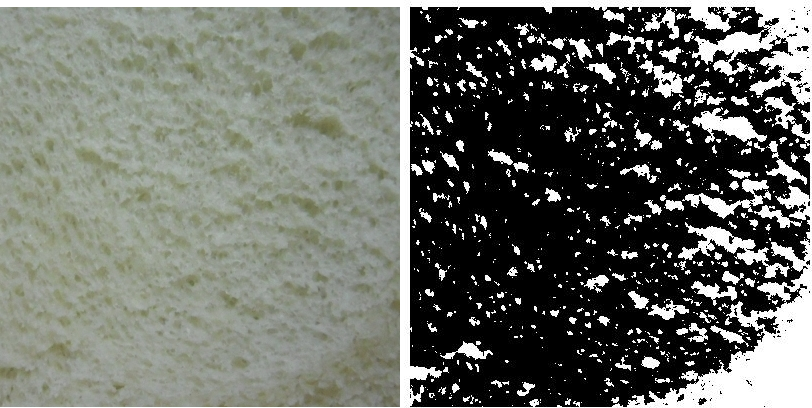
\includegraphics[width=11cm]{figures/segmal}
\caption[Imágen de pan binarizada utilizando umbralización global.]{Imágen de pan binarizada utilizando umbralización global. Al existir variaciones de iluminación en la imagen, la misma se binariza de manera incorrecta.}
\label{fig:segmal}
\end{figure}


La lógica del algoritmo de umbralización local se describe a continuación.
En cada píxel, el resultado de la binarización se computa a través de un promedio de los niveles de gris en una ventana que rodea ese píxel. Este promedio se compara con un umbral definido por el nivel de gris del píxel actual multiplicado por un número de sesgo ($bias$) y en caso de ser mayor, el píxel resultará blanco (en otro caso, negro), es decir:
\begin{equation}
\frac{\sum_{x,y \in W} f(x,y) }{W_{tam}} \geq f(x_{c},y_{c}) \times bias,
\label{eqn:white}
\end{equation}
donde $x_{c},y_{c}$ son las coordenadas del píxel actual y  $W$ es la ventana que rodea al píxel. Los dos parámetros que definen al algoritmo son: el tamaño de la ventana ($W_{tam}$) y el $bias$. 

Experimentalmente encontramos que estos parámetros dependen del método de captura utilizado. Los valores más adecuados para las muestras de escáner fueron $80$ para el tamaño de la ventana y $1.15 $ para el sesgo. En el caso de las muestras tomadas con una cámara digital, los valores óptimos fueron $80$ para la ventana y $1$ para el sesgo.  Estas diferencias parecen ser causadas por las diferentes condiciones de iluminación presentes en las imágenes. Queda planteado como trabajo a futuro la determinación automática de estos parámetros.

Es posible comparar el algoritmo con otros más sofisticados.
El algoritmo Mean Shift \cite{Comaniciu2002} es un método iterativo de agrupamiento (clustering) el cual segmenta objetos en la imagen, permitiendo separar el fondo y binarizar la imagen.
La Fig.~\ref{fig:meanshift} muestra el resultado de realizar una binarización con Mean Shift.
Se observa cierta similaridad en el resultado con respecto al algoritmo de umbralización local presentado, siendo el primero un método más simple de implementar.

\begin{figure}[h!]
\centering
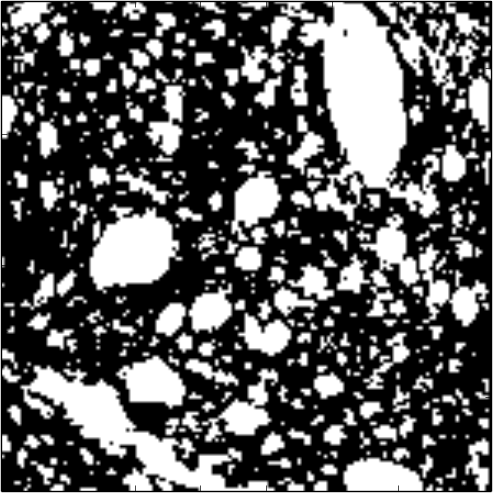
\includegraphics[width=4cm]{figures/meanshift}
\caption[Binarización utilizando el algoritmo Mean Shift.]{Binarización de la imagen izquierda de la Fig.~\ref{fig:bread}, utilizando el algoritmo Mean Shift. El resultado es similar al obtenido utilizando umbralización local.}
\label{fig:meanshift}
\end{figure}


En la Fig.~\ref{fig:bread} se observa una imagen con distintos tipos de panes (primera fila) y su binarización correspondiente, utilizando el algoritmo descripto (segunda fila).
Se removieron de la imagen binarizada elementos pequeños de $1$ o $2$ píxeles utilizando una operación de {\em opening} \cite{Gonzalez2006} (erosión seguida de dilatación) con un elemento estructurante de tamaño $2\times 2$ píxeles.
Las imágenes demuestran que este método presenta buenos resultados, incluso con condiciones de iluminación variando sobre la imagen.
En la Fig.~\ref{bin} puede observarse una imagen  y su binarizaci\'on.
La Fig.~\ref{fitbox} muestra los valores obtenidos en el c\'alculo de la dimensi\'on Box para esta imagen y la recta que ajusta estos valores. 
En la Fig.~\ref{fit} se observan los valores obtenidos por el algoritmo de Korcak para esta imagen y las rectas aproximantes (en la siguiente secci\'on se explica el por qu\'e de dos rectas aproximantes).


\begin{figure}[h!]
\centering
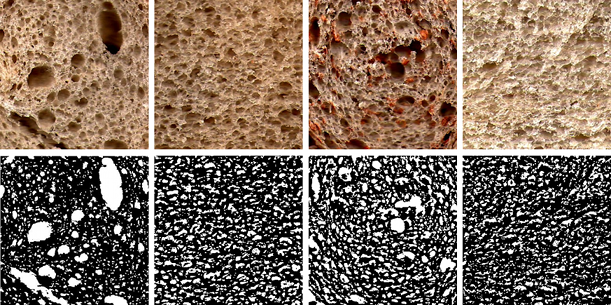
\includegraphics[width=12cm]{figures/binarizaciones}
\caption[Imágenes de distintos tipos de pan tomadas con un escáner.]{Imágenes de distintos tipos de pan tomadas con un escáner. {\em Baguette}, {\em lactal}, {\em salvado} y {\em sandwich} (primera fila) con sus correspondientes binarizaciones utilizando umbralamiento local (segunda fila).}
\label{fig:bread}
\end{figure}

\begin{figure}
\centering
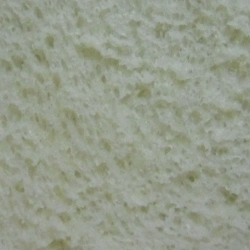
\includegraphics[width=5cm]{figures/lactal}
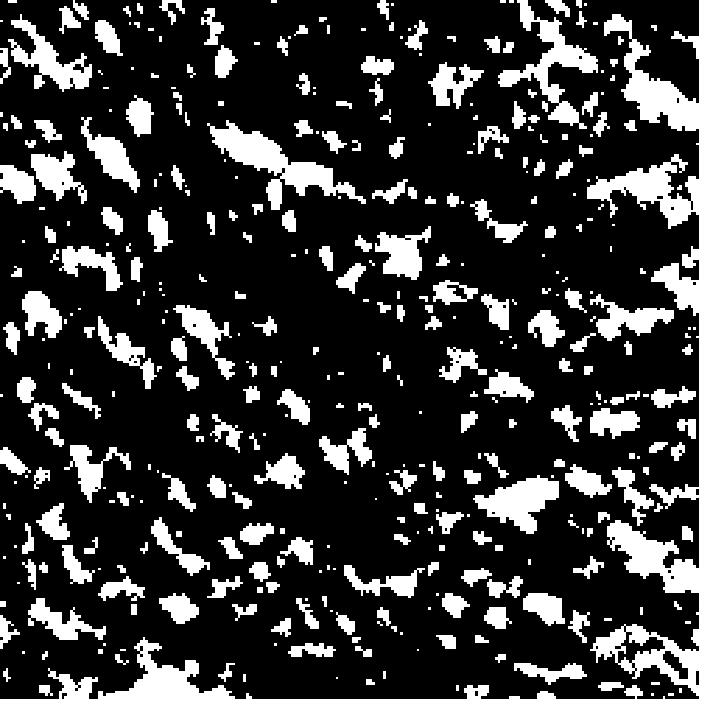
\includegraphics[width=5cm]{figures/lactalBin}
\caption{Imagen de un corte de pan (izquierda) y binarización (derecha), utilizando umbralización local.}
\label{bin}
\end{figure}

\begin{figure}
\centering
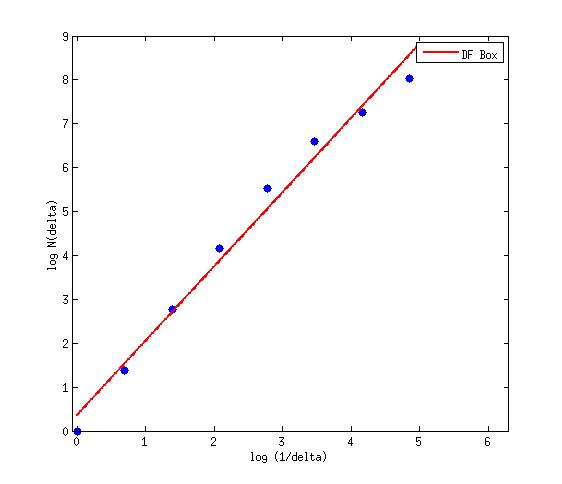
\includegraphics[width=8cm]{figures/fitbox}
\caption{Dimensi\'on Box de la imagen de la Figura \ref{bin}}
\label{fitbox}
\end{figure}


\begin{figure}
\centering
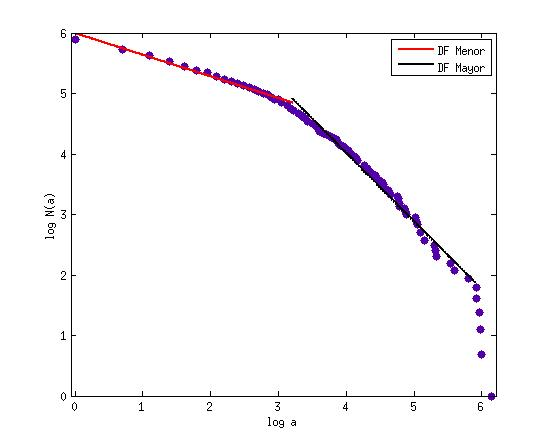
\includegraphics[width=8cm]{figures/lactal1PlotKorcak}
\caption{DFs de Korcak de la imagen de la Figura \ref{bin}}
\label{fit}
\end{figure}

\subsection{Dimensiones Estimadas}

En los diagramas $\log-\log $ obtenidos por los algoritmos (Korcak y DF Box), puede observarse que una \'unica recta no ajusta adecuadamente los valores. Esto sugiere que las muestras presentan caracter\'isticas {\em multifractales} \cite{Mandelbrot1989}.
Esto implica que se puede computar m\'as de una DF para la misma imagen. Se realizaron pruebas con pan lactal y mignon. Las DFs encontradas se incluyen en la Tabla \ref{tab:korcak}.

\begin{table}
\center
\begin{tabular}{|| l | l | l ||}
    \hline
     & DF (menor) & DF (mayor) \\    
    \hline
    Lactal 1 & 0.7152 & 2.214 \\
    \hline
    Lactal 2 & 0.8638 & 2.182 \\
    \hline
    Lactal 3 & 0.7598 & 2.046 \\
    \hline
    Lactal 4 & 0.8656 & 2.598 \\
    \hline
    Mignon 1 & 0.5068 & 1.1452\\
    \hline
    Mignon 2 & 0.4214 & 1.1608\\
    \hline
\end{tabular}
\caption{DFs de Korcak estimadas en muestras reales de pan}
\label{tab:korcak}
\end{table}

Para la regresi\'on por DF Box, los valores que se obtuvieron se muestran en la Tabla \ref{tab:box}.
Si bien se observa cierta similitud entre los valores obtenidos, se puede observar que la recta no ajusta perfectamente los datos en la figura.
De hecho, podrían utilizarse también dos rectas aproximantes buscando obtener un ajuste más preciso de los datos.

\begin{table}
\begin{center}
\begin{tabular}{|| l | l | l ||}
    \hline
     & DF \\    
    \hline
    Lactal 1 & 1.692 \\
    \hline
    Lactal 2 & 1.761 \\
    \hline
    Lactal 3 & 1.743\\
    \hline
    Lactal 4 & 1.73 \\
    \hline
    Mignon 1 & 1.686 \\
    \hline
    Mignon 2 & 1.726 \\
    \hline
\end{tabular}
\caption{DFs Box estimadas en muestras reales de pan}
\label{tab:box}
\end{center}
\end{table}

\section[Características Multifractales del pan]{Caracterización y Clasificación de Imágenes de Pan Utilizando Características Multifractales.}

La sección anterior mostró que al intentar computar una DF para una imagen de pan, resulta difícil utilizar una única recta que ajuste adecuadamente los datos obtenidos.
La utilización de más de una recta de ajuste permite reducir los errores de las regresiones lineales.
Es decir, dentro de la imagen resulta más adecuado calcular más de una DF, dependiendo del tamaño de las burbujas en consideración, o del tamaño de la ventana donde se cuenta la cantidad de píxeles.
Esto implica que necesitamos más de una DF para caracterizar adecuadamente una muestra.
En otras palabras, la teoría multifractal podría arrojar resultados más precisos sobre la composición de burbujas en la miga del pan.

El análisis fractal y multifractal ha probado ser útil para capturar propiedades clave del material a representar.
Estas características han sido aplicadas con éxito en diferentes áreas, como por ejemplo medicina \cite{Andjelkovic2008,Yu2011} y clasificación de texturas \cite{Wendt2009}.
En el tópico de alimentos, estas técnicas se han aplicado en el estudio de tejidos de manzanas \cite{Mendoza2010}, partes del cuerpo de cerdos \cite{Serrano2012}, y también en chocolate, y superficies de calabazas y papas \cite{Quevedo2002}.
Por medio de diferentes procedimientos \cite{Gonzales2008,Peitgen2004}, es posible obtener distintas DF, donde cada una captura una propiedad diferente del material (por ejemplo, porosidad, rugosidad, etc.).
Esto implica que la utilización de más de una DF podría permitir caracterizar más adecuadamente un material que por medio de la utilización de una única DF.

El análisis de los datos resultantes del proceso de extracción de características puede ayudar a obtener propiedades pertinentes a la apariencia o estructura geométrica de materiales.
Esta información puede ser utilizada en medidas de calidad de las muestras reales y en la validación de representaciones sintéticas de los mismos.
En otras palabras, estos procesos pueden utilizarse para determinar si una imagen dada presenta las características observadas en ese material, permitiendo además definir parámetros de calidad sobre los mismos.
En \cite{Fan2006}, un test de calidad de migas de pan basado en filtros de Gabor fue desarrollado, obteniendo buenos resultados en la clasificación de muestras de mayor y menor calidad.
Sin embargo, se utilizó una base de datos limitada ($30$ imágenes).
Como fue dicho, en \cite{Gonzales2008}, se obtuvieron distintas características fractales para un único tipo de pan, sugiriendo que un vector de DFs sería capaz de agrupar, en una única representación, muchas de las propiedades importantes de la miga del pan.

En esta sección proponemos el empleo del Espectro Multifractal (Multifractal Spectrum en inglés, \acrshort{MFS}) \cite{Xu2009} para describir y clasificar diferentes migas de panes.
Una de las principales características del MFS la constituye su invariancia bi-Lipschitz, esto es, invariancia a transformaciones de perspectiva (cambios en el punto de vista), y deformaciones suaves de las texturas de las superficies.
Está demostrado que el MFS resulta localmente invariante a cambios afines en la iluminación.
Estas propiedades resultan útiles para describir estructuras de migas de panes de una manera robusta y adecuada para los propósitos de esta sección.

La clasificación de texturas de alimentos ha sido abordada utilizando fractales y otras técnicas en \cite{Zong2010,Bosch2011}, pero estos trabajos no tienen en cuenta el esquema intra-clase, es decir, la clasificación se realiza entre diferentes alimentos, y no entre imágenes del mismo alimento.
En esta sección comparamos los MFS de distintos tipos de panes con otras características del estado del arte utilizando distintos clasificadores, estudiando además las correlaciones entre las características fractales obtenidas con el procedimiento y diferentes características estándares (heterogeneidad, porosidad y granularidad).

Además, se comparan las características fractales obtenidas, con el estado del arte en extracción de características para clasificación de texturas.
Los resultados de este procedimiento de extracción de características muestran que el clasificador presenta robustez y buenas propiedades de discriminación que le permiten distinguir entre diferentes tipos de panes y también la distinción de pan de imágenes de otros objetos.

\subsection{Teoría del Análisis Multifractal de Imágenes}
%\label{sec:4}

El análisis multifractal examina el límite en el comportamiento local de una medida $\mu$ en cada punto del conjunto en estudio.
Sea $E$ una estructura dividida en sub-estructuras disjuntas $E_{j}$ de tamaño $\varepsilon$ de tal manera que

\begin{equation}
\displaystyle\bigcup_{j}E_{j} = E.
\end{equation}

Cada sub-estructura $E_{j}$ está caracterizada por una medida $\mu(E_{j})$.
Definimos el exponente de H\"older, $\alpha$, para cada sub-estructura $E_{j}$, en función de $\varepsilon$, como el siguiente límite,


\begin{equation}
\alpha_{j} \triangleq \lim_{\varepsilon \rightarrow 0}{\frac{ln(\mu(E_{j}))}{ln(\varepsilon)} },
\label{eq:holder}
\end{equation}
\noindent

El límite $\alpha_{j}$ representa el valor del exponente de H\"older en un punto de la estructura, el cual caracteriza la regularidad local de la estructura en un punto.
Para obtener una caracterización global de la regularidad de la estructura se necesita obtener la distribución de $\alpha$ en $E$.
Luego, el espectro multifractal asociado al valor $\varepsilon$, $f_{\varepsilon}(\alpha)$, se obtiene contando las $N_{\varepsilon}$ cajas caracterizadas por poseer el mismo $\alpha$ de la siguiente manera,

\begin{equation}
f_{\varepsilon}(\alpha) = - \frac{ln(N_{\varepsilon}(\alpha = \alpha_{j}))}{ln(\varepsilon)}
\label{eq:eqn6},
\end{equation}

\noindent de esa forma queda definido $f_{\varepsilon}(\alpha)$ como el cociente entre los logaritmos de la cantidad de cajas que contienen al menos una sub-estructura cuyo $\alpha$ es $\alpha_{j}$.
Cuando $\varepsilon$ tiende a $0$, el valor límite se define como la dimensión fractal de la estructura $E$ caracterizada por $\alpha$ (la dimensión de Hausdorff de la distribución de $\alpha$).
También conocida como espectro {\em multifractal} $f(\alpha)$ (MFS) \cite{Silvetti2010}, es decir

\begin{equation}
f(\alpha) = \lim_{\varepsilon\to0}{f_{\varepsilon}(\alpha)}.
\label{eq:mfs}
\end{equation}

\subsubsection{Procedimiento práctico para computar el MFS en imágenes}
Existen diversas maneras, descriptas en la literatura, para obtener computacionalmente el MFS de una estructura.
Las mismas computan diferentes representaciones de la información multifractal presente en la estructura.
El método de momentos es el más utilizado \cite{Mendoza2010,Serrano2012}, pero el mismo produce un vector de características que no siempre resulta adecuado para realizar tareas de clasificación.
En esta sub-sección describiremos un procedimiento para implementar el método propuesto en \cite{Xu2009}, debido a sus resultados superiores en la clasificación.

El desarrollo de la sección anterior permite deducir un procedimiento para computar el MFS en una imagen.
En primer lugar se debe computar la regularidad local en cada píxel, para esto, se computa el exponente de H\"older, $\alpha_{x}$, para cada píxel $x$ de la imagen, utilizando la ecuación (\ref{eq:holder}).
Esto se logra definiendo a $B(x,\varepsilon)$ como el disco cerrado de radio $\varepsilon > 0$ centrado en $x$, y luego se reemplaza el límite en la ecuación con el ajuste lineal de los valores $log(\mu(B(x,\varepsilon)))$ y $log(\varepsilon)$.
Al aplicar este procedimiento en cada píxel, se obtiene lo que se denomina una $\alpha-$imagen, compuesta por un conjunto discreto de valores con un mínimo $\alpha_{min}$, y un máximo $\alpha_{max}$.
Para caracterizar globalmente la estructura, se debe aproximar la función que representa el MFS.
Debido a que la función tiene un dominio continuo, a fines prácticos se lo discretiza por medio de un conjunto de valores $\alpha_{i} \in [\alpha_{min},\alpha_{max}], \{\alpha_{i}, i = 1,\dots,M\}$, donde el conjunto de puntos que corresponde a un $\alpha_{i}$ se forma agrupando los píxeles de la $\alpha-$imagen cuyo valor está cerca a ese $\alpha_{i}$ bajo cierto umbral. 
Entonces, se aproxima la ecuación (\ref{eq:mfs}) por medio de un conjunto de DFs, donde cada DF corresponde a un $\alpha_{i}$.
Cada DF se computa por medio de la pendiente de la recta de ajuste entre los valores $log((N_{\varepsilon}(\alpha_{i}))$ y $log(\varepsilon)$. 
El valor $M$ determina el largo del vector, es decir, el número de FDs del MFS.

Como fue previamente aclarado, el espectro $f(\alpha)$ (MFS) y el método de momentos producen vectores que contienen la misma información.
En esta sección utilizamos la primera representación ($f(\alpha)$), ya que la misma produce una representación más adecuada que el método de momentos para tareas de clasificación.
Este proceso tiene como resultado un vector de características finito, el cual será utilizado posteriormente.
La cantidad de DFs del vector a utilizar será analizada posteriormente.


\subsubsection{Medidas Multifractales en imágenes}
\label{sec:mfsmeasures}
Las funciones $\mu$ son definidas intentando capturar determinadas características de las imágenes.
El primer ejemplo consiste en definir $\mu$ en el dominio de intensidades de la imagen (I), es decir

\begin{equation}
\mu(B(x,\varepsilon)) = \int_{B(x,\varepsilon)}{(G_{\varepsilon} \ast I)} dx,
\label{eqn:eqn11}
\end{equation}
\noindent donde $\ast$ representa el operador de convolución $2D$ y $G_{\varepsilon}$ un kernel Gaussiano con variancia $\varepsilon$, en otras palabras $\mu$ es el promedio ponderado de los valores de intensidades en el disco de radio $\varepsilon$ centrado en $x$ ($B(x,\varepsilon)$).
Esta función se define como la densidad de la intensidad, y describe como la intensidad se modifica en un punto con la escala.

La definición de $\mu$ puede ser realizada con fines específicos.
Por ejemplo, si se requiere robustez ante los cambios de iluminación, una opción consiste en definir $\mu(B(x,\varepsilon))$ en el dominio de la energía de los gradientes.
Sean ${ f_{k} , k = 1, 2, 3, 4}$ cuatro operadores diferenciales en las direcciones vertical, horizontal, diagonal y anti-diagonal respectivamente.
Se define una función de medida $\mu(B(x,\varepsilon))$ para la imagen $I$ como sigue:

\begin{equation}
\mu(B(x,\varepsilon)) = (\int_{B(x,\varepsilon)}{\sum_{k}{(f_{k} \ast (G_{\varepsilon} \ast I))^{2}} dx)^{1/2}}.
\label{eqn:gradient}
\end{equation}

Otra elección consiste en definir $\mu(B(x, \varepsilon))$ como la suma de los laplacianos de la imagen dentro de $B(x, \varepsilon)$, es decir

\begin{equation}
\mu(B(x,\varepsilon)) = \int_{B(x,\varepsilon)}|\nabla^2 (G_{\varepsilon} \ast I)| dx.
\label{eqn:laplacian}
\end{equation}

\subsection{Procedimiento de captura de imágenes de pan}
En las siguientes subsecciones realizaremos pruebas con el MFS como vector de características de imágenes de distintos tipos de pan.
Para esto primero obtuvimos muestras reales de imágenes de cortes del material.
Se obtuvieron $20$ imágenes de $4$ tipos de panes diferentes ({\em baguette}, {\em lactal}, {\em salvado} y {\em sandwich}, contabilizando $80$ imágenes) utilizando un escáner HP PSC 1210 con los siguientes parámetros de captura:  highlight $190$, shadows $40$, and midtones $1$.
Las imágenes fueron obtenidas a una resolución de $380\times 380$ píxeles (el área máxima posible para los $4$ tipos de pan) a una resolución de $350$ dpi ($1$ pixel $= 0.00527$ $[mm^{2}]$).
Las mismas fueron convertidas a escala de grises ($8$ bits).
Además, se obtuvieron $20$ imágenes de cada tipo de pan utilizando una cámara digital con la misma resolución espacial.
Las condiciones de iluminación de estas imágenes son distintas a las de las imágenes del escáner, con el propósito de mesurar la robustez del método.
En la Figura ~\ref{fig:camera} se observan $4$ ejemplos de imágenes de pan obtenidas con la cámara digital. Además se utilizaron $40$ imágenes de la base de imágenes CalTech101 dataset~\cite{FeiFei04} para introducir imágenes de objetos diferentes al pan y observar la capacidad del método para separar panes de otros objetos.

\begin{figure}[h!]
\centering
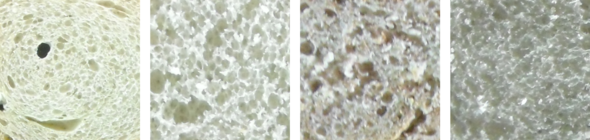
\includegraphics[width=12cm]{figures/pancamara}
\caption{Imágenes de pan tomadas con una cámara digital.}
\label{fig:camera}
\end{figure}

\subsection{Extracción de Características de Migas de Panes}
Para obtener una mayor comprensión de los valores de las DF del método multifractal, se extrajeron características típicas de las imágenes binarizadas para establecer correlaciones con las dimensiones del MFS.
Se computaron la fracción de vacío de la imagen (\acrshort{VF}), el área media de las burbujas (\acrshort{MCA}) y el desvío estándar del área media de las burbujas (\acrshort{stCA}) con el propósito de establecer relaciones con la porosidad, granularidad y heterogeneidad de las diferentes migas.


\section{MFS como vector de características}

En esta sección nos proponemos demostrar el adecuado comportamiento del MFS como descriptor de imágenes de pan.
Computamos el MFS para cada una de las $200$ imágenes presentes en la base de datos ($40$ imágenes de cada tipo, incluyendo no-pan), obteniendo $5$ clases balanceadas.
En las siguientes subsecciones analizaremos los datos obtenidos, además de utilizarlos en la clasificación de las muestras.

\subsection{Análisis del MFS de las imágenes de pan y otros objetos}

Los Mapas Auto-Organizados (Self-Organising Maps -  \acrshort{SOM})~\cite{Kohonen2001} son herramientas de aprendizaje no supervisado que permiten reducir la dimensionalidad de un conjunto de datos para comprender su relación espacial.
Los mapas SOM mapean datos multidimensionales en $2$ dimensiones utilizando información de vecindad, preservando así la información topológica de los mismos.

La Figura~\ref{fig:somfractal} muestra el  SOM de las representaciones multifractales de las imágenes de pan y de no-pan en una grilla de $10\times 10$ (el comportamiento resulta similar para distintos tamaños de grilla).
La imagen de la izquierda muestra las $5$ clases ({\em baguette}, {\em lactal}, {\em salvado}, {\em sandwich} y {\em no-pan}).
En la imagen de la derecha la clase {\em no-pan} fue removida y el SOM recomputado para las restantes $4$ clases, con la intención de observar más detenidamente la relación entre los MFS de las distintas clases de pan.
Las imágenes muestran, a primera vista, clases fácilmente separables.
Un clasificador podría determinar regiones del espacio y clasificar de manera adecuada las clases, ya que se encuentran claramente separadas unas de otras (no existen prácticamente celdas con más de un número de clase en ellas).
En la Figura~\ref{fig:boxplotsMFS}, se muestran boxplots del MFS de los cuatro tipos de panes con la mediana de cada dimensión (en rojo) unida por una línea a trozos.
Cada dimensión fractal corresponde a un valor de $\alpha_{i}$.
En nuestros experimentos el vector de MFS contiene $20$ dimensiones fractales. De estos datos se infiere que la primer mitad del MFS (primeras $10$ DFs, $\alpha \in [0: 0.53)$), la dispersión resulta mayor que en la segunda mitad del espectro  (últimas $10$ DFs, $\alpha \in [0.53: 1]$).
Es decir, la segunda mitad del espectro puede identificar cada tipo de pan.


\begin{figure}[h!]
\begin{centering}
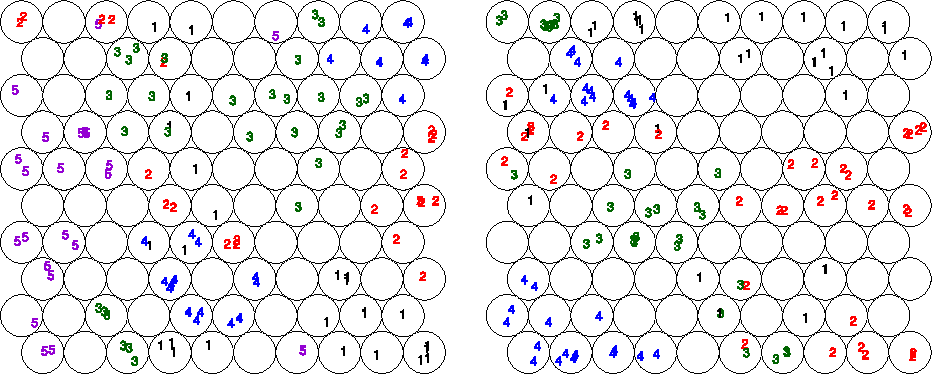
\includegraphics[width=12cm]{figures/SOM}
\caption[Mapas Auto-Organizados de imágenes de panes y otros objetos]{Mapas Auto-Organizados (Self-Organising Maps SOM). SOM de imágenes de panes y no-panes (izquierda) y SOM sólo de tipos de panes (derecha). $1$: {\em baguette}, $2$: {\em lactal}, $3$: {\em salvado}, $4$: {\em sandwich}, $5$: {\em no-pan}.}
\label{fig:somfractal}
\end{centering}
\end{figure}

\begin{figure}[h!]
\centering
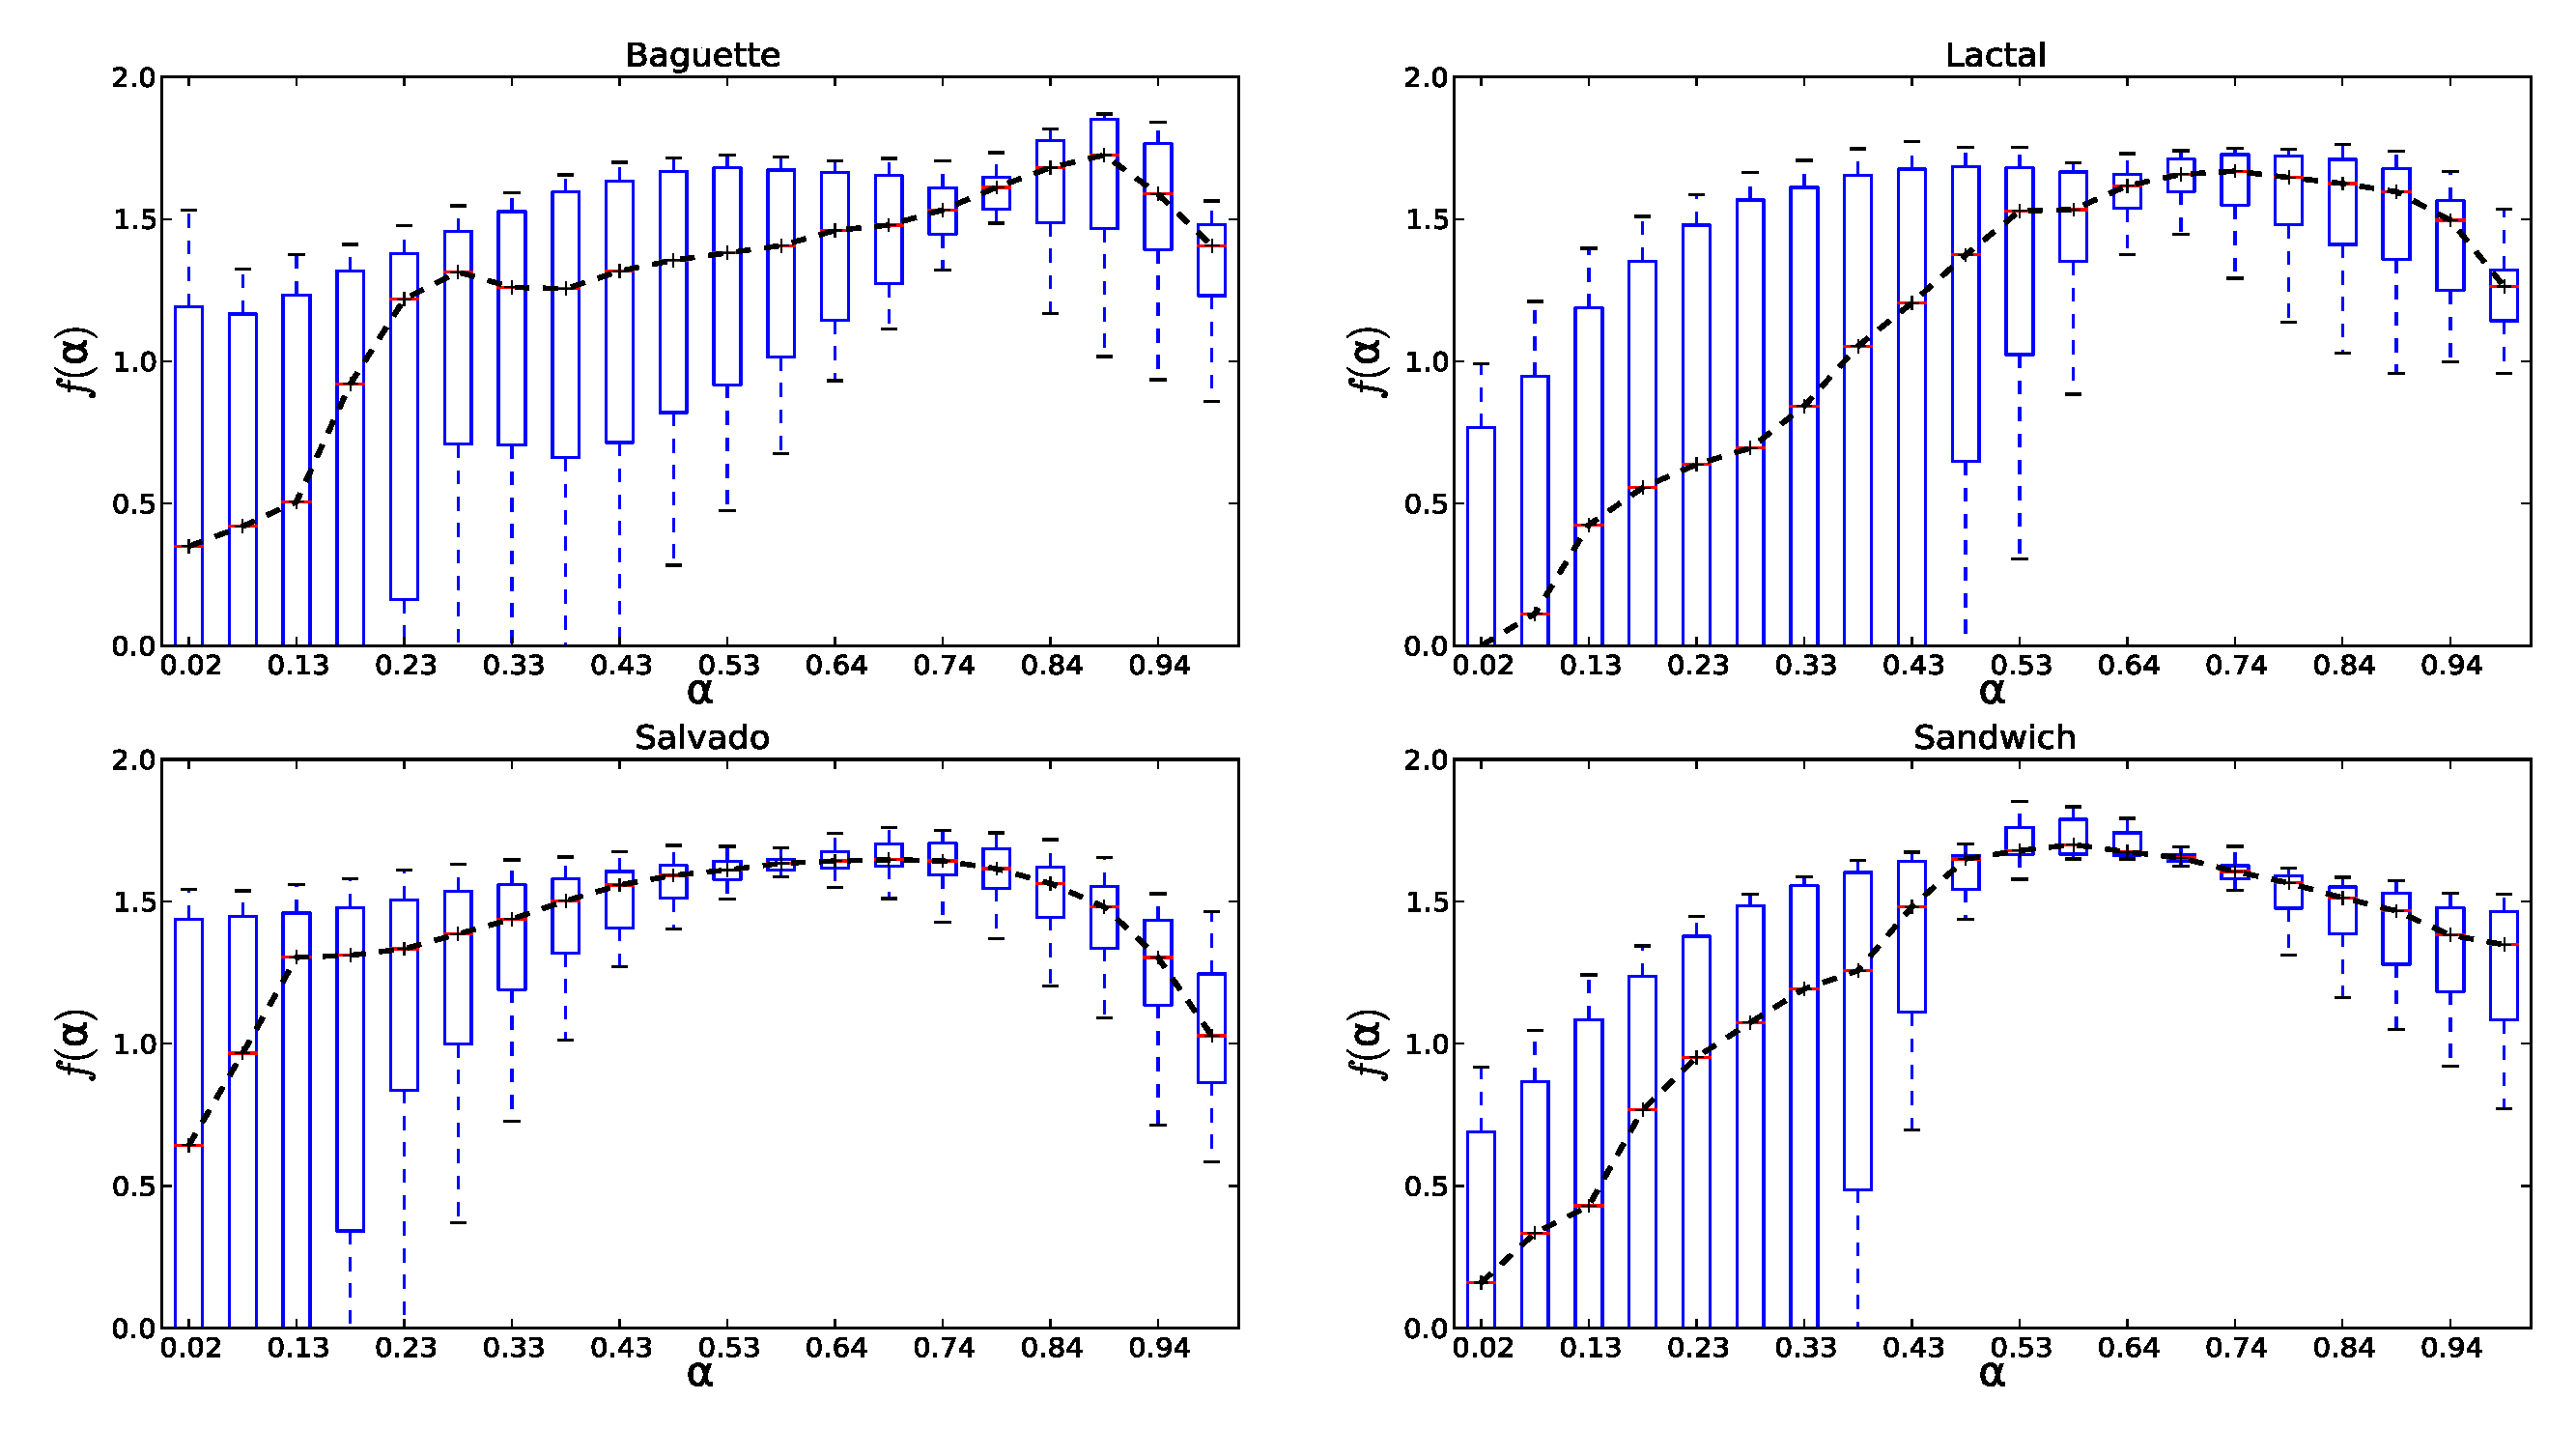
\includegraphics[width=12cm]{figures/boxplots}
\caption[Boxplots de distintos tipos de panes]{Boxplots de cuatro tipos de panes comunes. Las medianas de las dimensiones se unen con una línea a trozos. Arriba: {\em baguette} (izquierda), {\em lactal} (derecha), abajo: {\em salvado} (izquierda), {\em sandwich} (derecha).}
\label{fig:boxplotsMFS}
\end{figure}


Los datos muestran que cada tipo de pan posee una curva característica en este sector del espectro, pero esta curva se modifica si se modifican las condiciones de iluminación (es decir, si se toma con el escáner o la cámara), en otras palabras esto altera el MFS obtenido, y por lo tanto no poseemos un único MFS para cada tipo de pan. 
Por completitud, en la Figura~\ref{fig:meansMFS}, mostramos la media y el desvío estándar del MFS de cada tipo de pan.
La imagen muestra, al igual que en los casos anteriores, que el MFS puede ser aprovechado para separar diferentes tipos de pan, ya que los valores medios de cada clase son distintos.


\begin{figure}[h!]
\centering
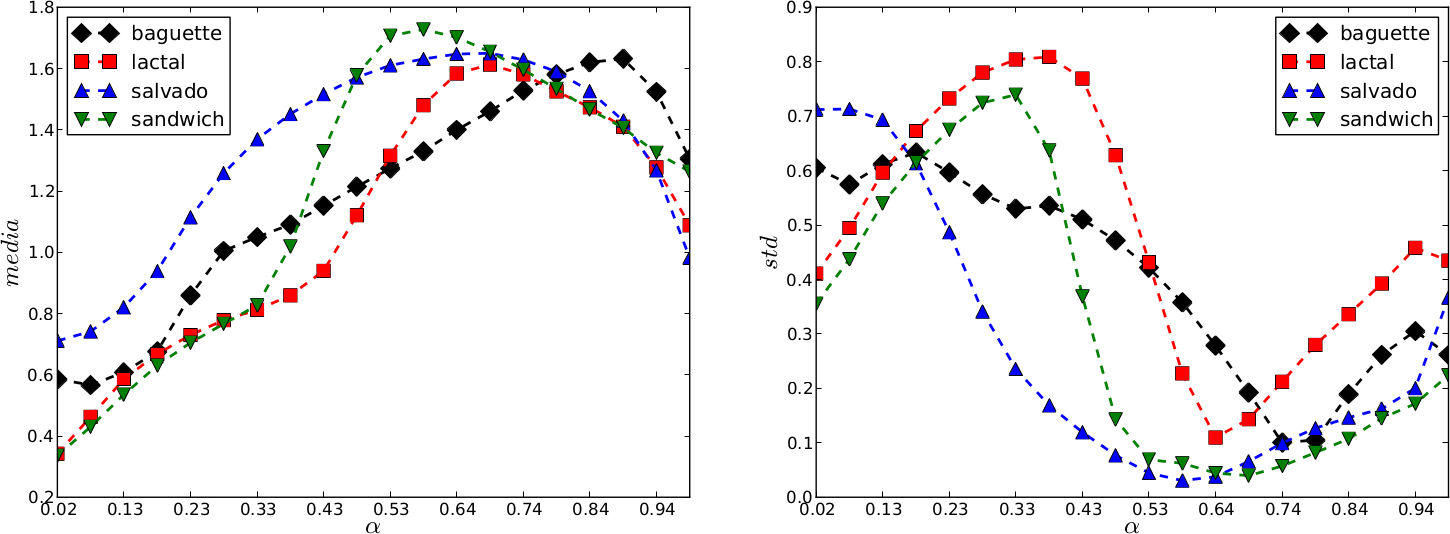
\includegraphics[width=12cm]{figures/panstd}
\caption[MFS promedio y desvíos estándar de las FDs para los cuatro tipos de panes]{MFS promedio y desvíos estándar de las FDs para los cuatro tipos de panes. Izquierda: MFS promedio, derecha: desvíos estándar.}
\label{fig:meansMFS}
\end{figure}

\subsection{Correlación entre Dimensiones Fractales y Características de la Miga de Pan.}

Computamos además el coeficiente de correlación de Spearman ($\rho$) para los cuatro tipos de pan, entre cada dimensión fractal del espectro y la fracción de vacío, el área media de burbuja y el desvío estándar del área media de burbuja (en $[mm^{2}]$), los cuales pueden observarse en las Figuras \ref{fig:corrVF}, \ref{fig:corrMCA} y \ref{fig:corrMCAstdev}, respectivamente, como una función de la dimensión fractal.
Solamente las muestras de escáner fueron tenidas en cuenta en las correlaciones, para obtener información más precisa en el análisis.
Preferimos $\rho$ al coeficiente de Pearson $R$ ya que el primero no asume una dependencia lineal para exhibir correlaciones en los datos.

La Figura~\ref{fig:corrVF} muestra que los coeficientes de las primeras $5$ dimensiones se comportan similarmente ($\alpha \in [0: 0.23]$) en todos los tipos de pan y de manera distinta para la dimensión $5$ y superiores. Esto quiere decir que las primeras $5$ dimensiones están altamente correlacionadas con la fracción de vacío (porosidad) de las muestras escaneadas.
Esto significa que las primeras DFs crecen cuando la fracción de vacío crece.
Si bien otras dimensiones presentan correlaciones estadísticamente relevantes, lo mismo sólo ocurre en determinados tipos de pan, por lo cual el resultado depende del tipo de pan que se considere.
De las imágenes correspondientes a los coeficientes de correlación MCA y stCA (Figuras \ref{fig:corrMCA} y \ref{fig:corrMCAstdev} respectivamente) se desprende que el área media de burbujas está más correlacionada con las dimensiones fractales que el desvío estándar del área media de burbujas. Esto significa que la granularidad de la miga de pan puede ser caracterizada de manera más precisa con el MFS, que su heterogeneidad.


\begin{figure}[h!]
\centering
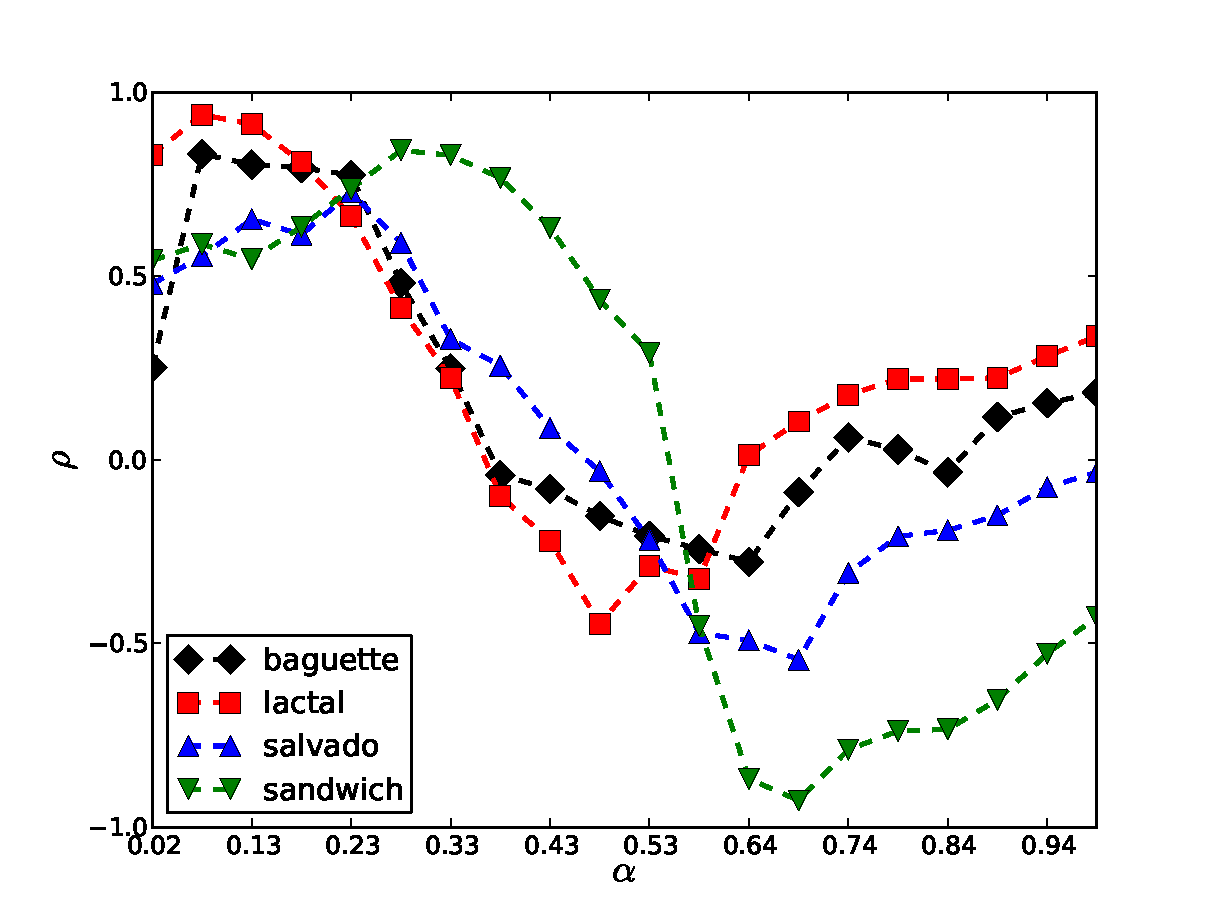
\includegraphics[width=8cm]{figures/VF}
\caption{Coeficiente de correlación Spearman entre las FDs del MFS y la fracción de vacío (VF) de las muestras escaneadas.}
\label{fig:corrVF}
\end{figure}

\begin{figure}[h!]
\centering
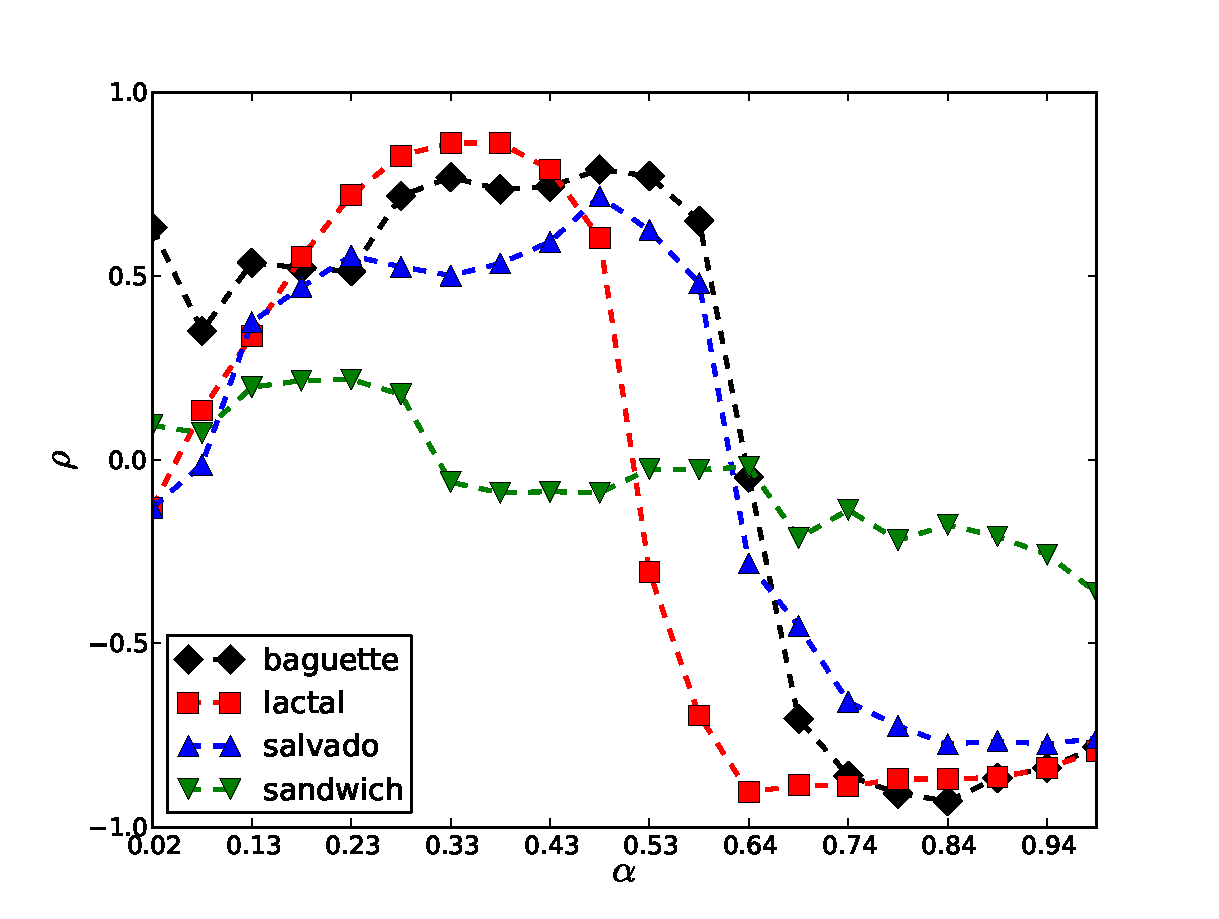
\includegraphics[width=8cm]{figures/MCA}
\caption{Coeficiente de correlación Spearman entre las FDs del MFS y el área media de las burbujas (MCA) de las muestras escaneadas. (en $[mm^{2}]$).}
\label{fig:corrMCA}
\end{figure}

\begin{figure}[h!]
\centering
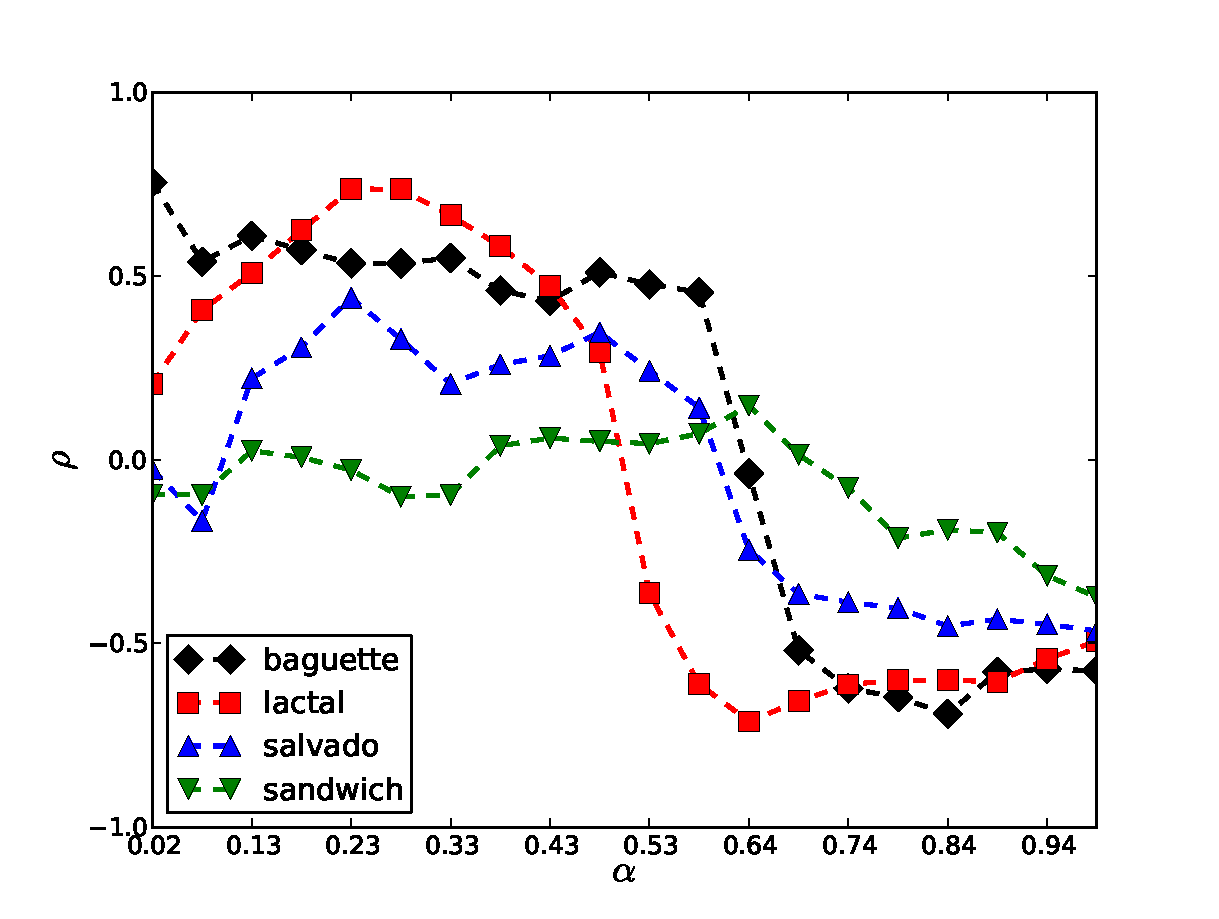
\includegraphics[width=8cm]{figures/stMCA}
\caption{Coeficiente de correlación Spearman entre las FDs del MFS y el desvío estándar del área media de las burbujas (stCA) de las muestras escaneadas. (en $[mm^{2}]$).}
\label{fig:corrMCAstdev}
\end{figure}

Adicionalmente, las últimas $5$ dimensiones fractales  del espectro ($\alpha \in [0.79: 1]$) están también (pero de manera inversa) correlacionadas con el MCA de las burbujas.
Esto quiere decir que las DFs se incrementan cuando el MCA se decrementa.
La misma observación puede realizarse para el stCA, pero las correlaciones son menores.
En ambos casos, los coeficientes de correlación de la clase {\em sandwich} son los menores entre todos los tipos de pan considerados.

Resumiendo, las dimensiones del MFS que corresponden a valores de  $\alpha \in [0: 0.23]$ son útiles para medir la porosidad de las muestras escaneadas. Además, granularidad y heterogeneidad pueden ser medidas por las dimensiones con  $\alpha \in [0.79: 1]$.
Es decir, con un único vector de dimensiones fractales medimos diferentes características claves de la miga de pan, como fue sugerido en \cite{Gonzales2008}.

\subsection{Clasificaci\'on de imágenes de diferentes tipos de pan}

Definimos $5$ clases {\em baguette}, {\em lactal}, {\em salvado}, {\em sandwich} y {\em no-pan}, asignando $40$ imágenes a cada clase.  Se establecen comparaciones además entre el MFS y métodos del estado del arte en visión por computadora.
Este esquema de clasificación corresponde a un esquema intra-clase (donde cada clase representa un tipo distinto del mismo objeto), el cual resulta más dificultoso de resolver que un esquema inter-clase (donde cada clase representa un objeto distinto).

Se aplica K-fold cross-validation a todo el conjunto (con $K=4$), utilizando tres clasificadores distintos: Máquinas de vectores de soporte (Support Vector Machines, \acrshort{SVM}),  bosques aleatorios (Random Forests, \acrshort{RF}) \cite{Breiman2001}, y vecinos más cercanos (Nearest Neighbors, \acrshort{NN}).
Los resultados muestran que el MFS realiza una muy buena clasificación independientemente del clasificador utilizado.
La implementación de SVM utilizada fue \textsf{libsvm} \cite{Chang2011} (con kernel RBF).
Se utilizó la librería python \textsf{scikit-learn} en los restantes algoritmos de clasificación.
En el caso de RF, se utilizaron $100$ árboles y en NN, un vecino.
En la Tabla~\ref{tab:number}, se observan los resultados del método utilizando diferente número de FDs.
Una combinación práctica de rendimiento y baja dimensionalidad se alcanza al utilizar $20$ FDs (en ese caso se obtienen los resultados de mejor desempeño para los algoritmos de clasificación RF y NN), por lo tanto este número de FDs se utilizará en las computaciones subsiguientes.


\begin{table}[h!]
\center
\begin{tabular}{lllll}
\hline\noalign{\smallskip}
\#FDs & 10  & 20 & 30 \\
\noalign{\smallskip}\hline\noalign{\smallskip}
SVM & \textbf{96\%} & 94.5\% & 95.5\% \\
RF  & 91.5\% & \textbf{93.5\%} & 93\% \\
NN & 88.5\% & \textbf{90.5\%} & 90\% \\
\noalign{\smallskip}\hline
\end{tabular}
\caption{Resultados de la clasificación de migas de pan utilizando diferente número de características para el MFS y diferentes algoritmos de clasificación.}
\label{tab:number}       % Give a unique label
\end{table}


La Tabla \ref{tab:mfs} muestra el rendimiento de diferentes combinaciones de diferentes MFS.
El MFS utilizado en este estudio fue computado basado en la densidad de la intensidad (MFS en la Tabla), el laplaciano de la intensidad (L), y el gradiente de la intensidad (G) (ver sección \ref{sec:mfsmeasures}).
Además, se llevó a cabo un experimento utilizando el espacio de color CIELab \cite{Hunter58}, debido a que el mismo tiende a reducir la dependencia del color resultante de la imagen con respecto al dispositivo de captura utilizado.
Las imágenes son transformadas a dicho espacio, y el MFS de los tres canales separados ({\em L}, {\em a} y {\em b}) son agrupados para obtener un vector de $60$ FDs.
Luego mostraremos que esta combinación produjo los resultados de mejor desempeño en la clasificación.
Esto implica que añadir información de color representada en un espacio cromático diferente resultó útil para clasificar diferentes tipos de panes, donde se emplearon diferentes tipos de dispositivos de captura (en nuestro caso, un escáner y una cámara digital).



\begin{table}[h!]
\center
\begin{tabular}{lllll}
\hline\noalign{\smallskip}
Método & MFS & MFS+L & MFS+G & CIELab  \\
\noalign{\smallskip}\hline\noalign{\smallskip}
SVM & 94.5\% & 95.5\% & \textbf{97.5\%} & \textbf{97.5\%} \\
RF  & 93.5\% & \textbf{96\%} & 95\% & \textbf{96\%} \\
NN & 90.5\% & 90\% & 87\% & \textbf{92\%} \\
\noalign{\smallskip}\hline
\#FDs & 20 & 40 & 40 & 60 \\
\hline
\end{tabular}
\caption{Resultados de la clasificación de migas de pan utilizando diferentes combinaciones del MFS y diferentes algoritmos de clasificación.}
\label{tab:mfs}       % Give a unique label
\end{table}

La Tabla \ref{tab:other} muestra características del estado del arte: Haralick \cite{Haralick73}, patrón binario local \cite{Ojala96} (Local Binary Pattern, \acrshort{Lbp}), y característica de transformación invariante a escala \cite{Lowe2004} (Scale-invariant feature transform, \acrshort{SIFT}), las cuales son computadas en las imágenes.
La clasificación más alta se obtiene para las características SIFT, pero el método requiere un vector de $128$ características para cada imagen.
Además se requiere tiempo computacional y espacio de almacenamiento para construir determinadas estructuras utilizadas por el método (una estructura llamada {\em libro} de códigos, {\em codebook}).


\begin{table}[h!]
\center
% For LaTeX tables use
\begin{tabular}{llllll}
\hline\noalign{\smallskip}
Método & Haralick & Lbp & SIFT\\ % & Zernicke
\noalign{\smallskip}\hline\noalign{\smallskip}
SVM & 94\% & 78.5\% & \textbf{96.5\%} \\ % & 55 
RF  & 91\% & 71.5\% & \textbf{92\%} \\ % & 58 
NN & 79\% & 70\% & \textbf{86\%} \\ % & 48.5 
\noalign{\smallskip}\hline
\#FDs & 13 & 36 & 128 \\
\hline
\end{tabular}
\caption{Resultados de la clasificación de migas de pan para diferentes características del estado del arte y diferentes algoritmos de clasificación.}
\label{tab:other}       % Give a unique label
\end{table}


Para una mayor comprensión de los resultados, se pueden computar las matrices de confusión de los procedimientos.
Como ejemplo, el resultado de mejor desempeño se alcanza al utilizar el método CIELab, en conjunción al algoritmo de clasificación SVM.
La matriz de confusión correspondiente puede observarse en la Tabla \ref{tab:confusionmatrix}.


\begin{table}[h!]
\center
% For LaTeX tables use
\begin{tabular}{llllll}
\hline\noalign{\smallskip}
Clase&{\em baguette} & {\em lactal} & {\em salvado} &{\em sandwich}&{\em no-pan} \\
\noalign{\smallskip}\hline\noalign{\smallskip}
{\em baguette} & 39& 1 &1 &0 &0 \\
{\em lactal} & 0& 38 &0 &0 &0  \\
{\em salvado} & 0& 0 &39 &1 &0  \\
{\em sandwich} & 1& 1 &0 &39 &0  \\
{\em no-pan} & 0& 0 &0 &0 &40  \\
\hline
\end{tabular}
\caption{Matriz de confusión para los resultados de mejor desempeño (método CIELab, utilizando el algoritmo de clasificación SVM).}
\label{tab:confusionmatrix}       % Give a unique label
\end{table}

Cada columna de la matriz muestra los resultados de la clasificación de las $40$ imágenes de cada clase.
De la tabla se desprende que el método clasifica imágenes de manera incorrecta en muy pocos casos.
Por ejemplo, de las $40$ imágenes de pan lactal, sólo $2$ son clasificadas erróneamente, específicamente como {\em baguette} y {\em sandwich} (ver columna con encabezado {\em lactal}).
Las otras clases se comportan similarmente.
La diferenciación entre imágenes de pan y {\em no pan} no presenta errores, es decir, ninguna imagen de alguna de las clases de pan fue clasificada como {\em no pan} y viceversa.
La tabla muestra que el $97.5\%$ de la base de datos se clasifica correctamente ($5$ errores de $200$ posibles).

En la clasificación de la base de datos, el MFS obtiene el mejor desempeño entre los algoritmos estudiados.
El MFS captura información robusta en unos pocos valores.
Estos resultados concuerdan con los obtenidos en \cite{Bosch2011} para la clasificación de otros productos alimenticios.
Esta sección demostró la capacidad del MFS para caracterizar imágenes de cortes de la miga del pan, diferenciándola entre distintos tipos del mismo.
Los resultados pueden ser útiles en la caracterización de las cualidades de su estructura.
Además, la clasificación puede aplicarse en ambientes donde se trabaje con migas reales de panes.


%\begin{figure}[h!]
%\centering
%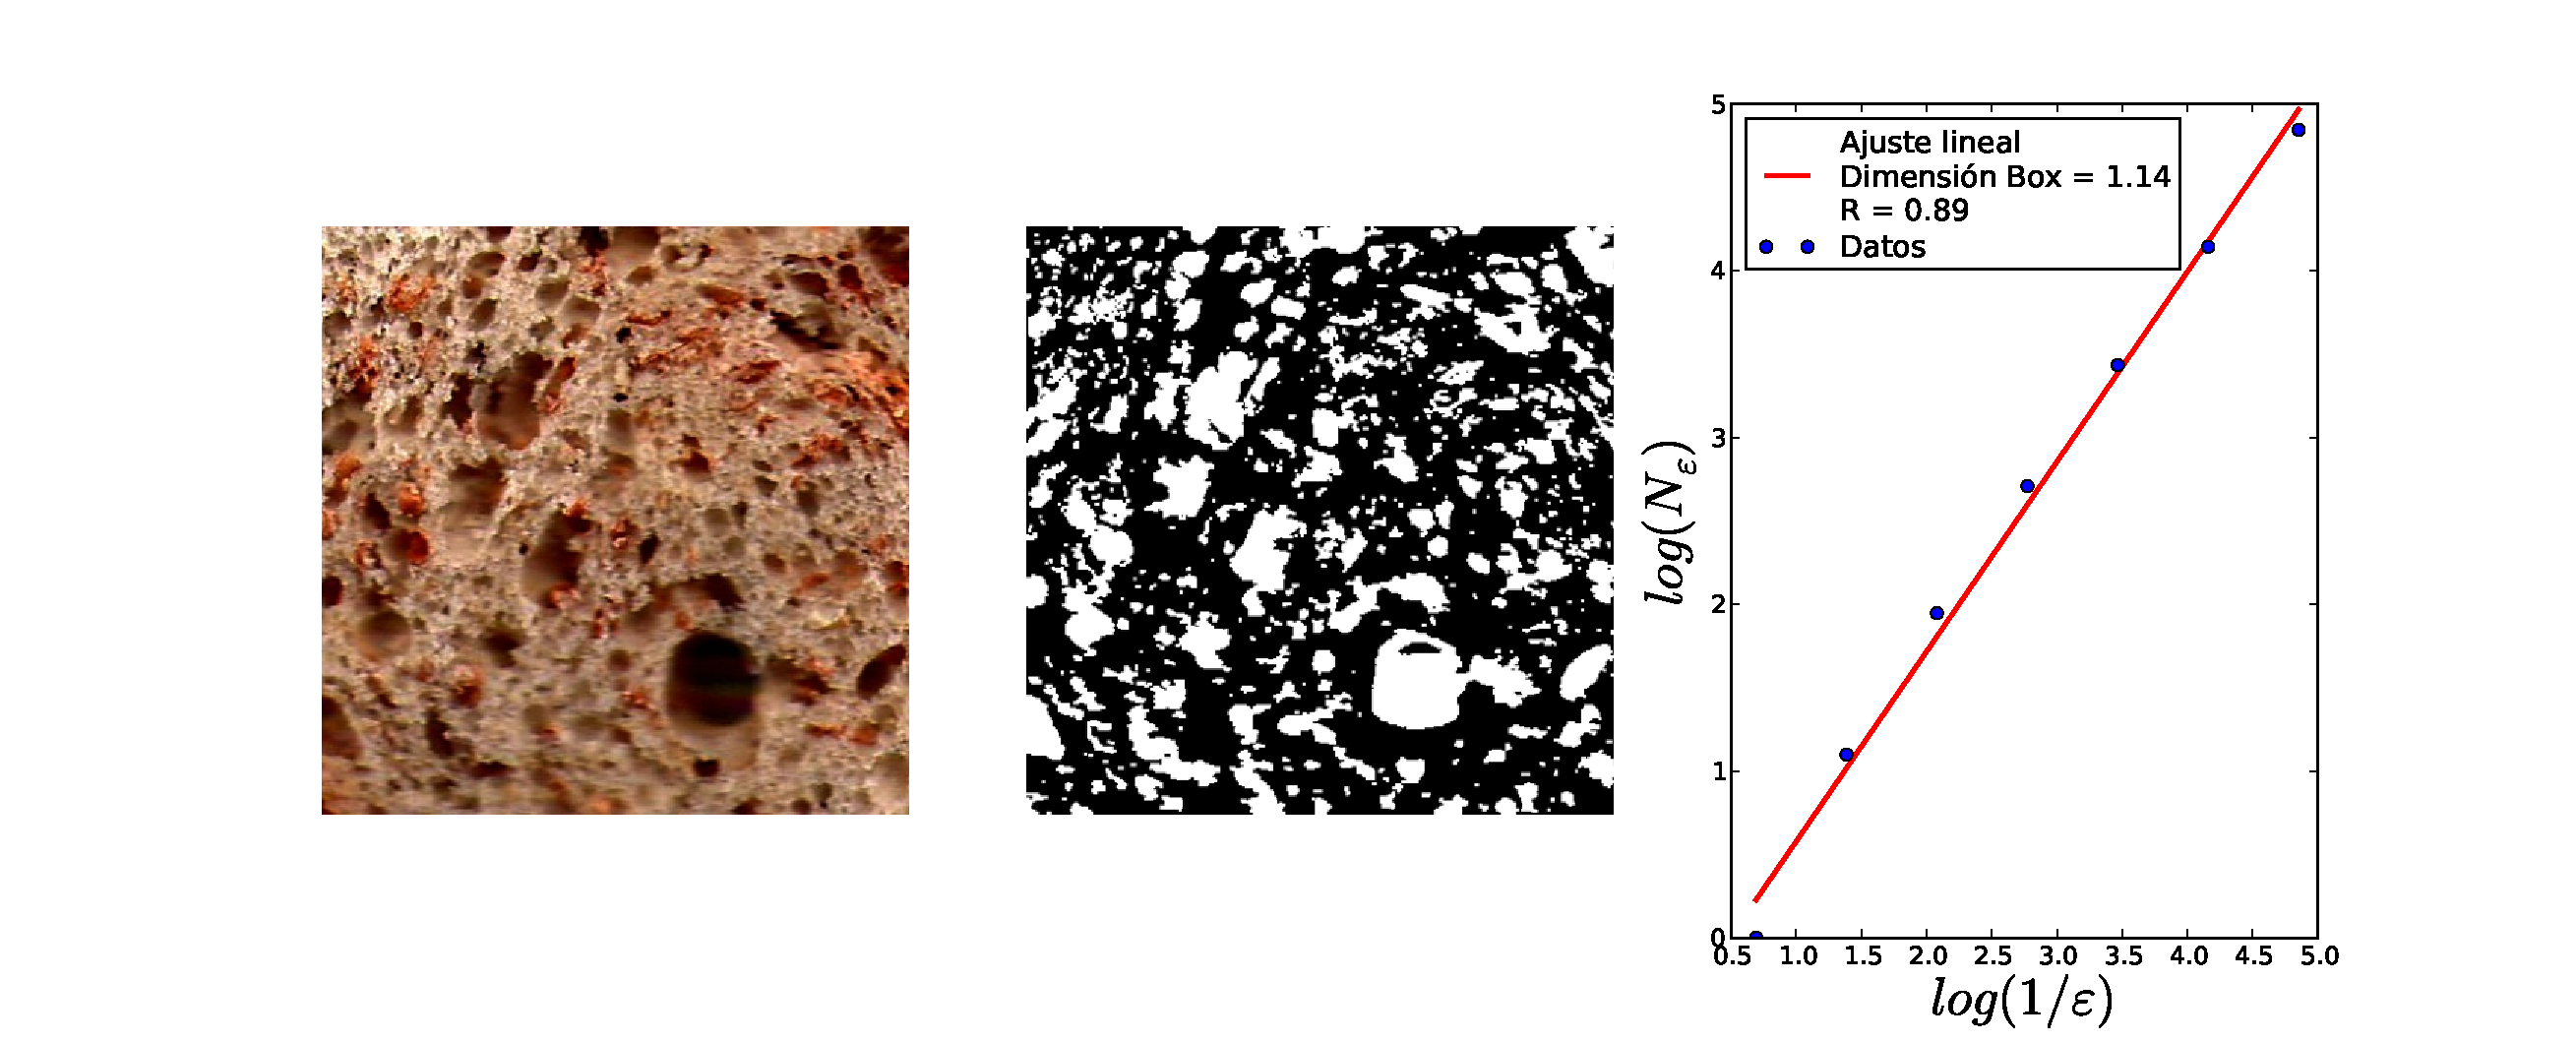
\includegraphics[width=14cm]{dimensionbox}
%\caption[Cómputo de la dimensión Box.]{Cómputo de la dimensión Box. Una imagen de pan (izquierda) con su binarización (centro) y su dimensión box computada (derecha).}
%\label{fig:fitbox}
%\end{figure}

\section{Validación de Imágenes Sintéticas de Pan}

En el capítulo de modelado introdujimos distintos algoritmos para modelar la geometría de la miga del pan.
En esta sección mostraremos que el algoritmo de modelado que atiende al proceso de fabricación del pan puede ser validado utilizando métodos multifractales.
Particularmente, utilizaremos el MFS previamente descripto, pero en otra representación, la cual resulta más adecuada para los propósitos de esta sección.
Esta forma de computar el MFS se utiliza ampliamente en análisis de texturas en visión por computadoras y en análisis de patrones.

A diferencia de las características fractales \cite{Gonzales2008}, la teoría multifractal ha sido utilizada para describir características de imágenes, pero no en caracterización de panes.
Existen dos clases principales de espectro multifractal: dimensiones generalizadas ($D_{q}$) y exponentes de Lipschitz-H\"older ($f(\alpha)$). 
La última representación resulta útil en clasificación, como fue mostrado.
Las dimensiones multifractales generalizadas pueden ser computadas de muchas maneras, de las cuales el método Sandbox \cite{Tel1989} calcula el valor medio de muchas muestras aleatoriamente distribuidas, sobre puntos pertenecientes a la estructura \cite{Debartolo2004}. 

La dimensión generalizada de orden $q$ con el método Sandbox se define como:

 \begin{align*}
D_{q\ne 1}^{sb} &= \frac{1}{q-1} \lim_{R \rightarrow 0}{
\frac{ln   { \left\langle  (M(R)/M_{0})^{q-1} \right\rangle   }}
{ln {(R/L)}       }},\\
D_{q=1}^{sb} &= \lim_{R \rightarrow 0}{
\frac{ \left\langle ln   { (M(R)/M_{0})  }  \right\rangle}
{ln {(R/L)}       }},
\end{align*}

\noindent donde $M_{0}$ es la cantidad de píxeles blancos en la imagen binarizada y $M(R)$ es el número de puntos que pertenecen a la estructura en un círculo de radio $R$ centrado en un punto de la misma.
Cuando $q\ne1$, computamos el límite como la pendiente del ajuste lineal de los valores $ln(R/L)$ vs. $ ln  \left\langle  { (M(R)/M_{0})^{q-1} }  \right\rangle$, para $R$ en $[R_{min}, R_{max}]$, donde $ \left\langle \cdot  \right\rangle$ denota el valor medio sobre los puntos muestreados.
Se procede similarmente para $q=1$. 
Computando el valor para diferentes $q \in [Q_{min},Q_{max}]$  se obtiene el espectro Sandbox.

Esta metodología para el cálculo del MFS aparece reportada como la más adecuada para análisis de características texturales y geométricas \cite{Gonzales2008}, por lo que la utilizamos sobre $10$ imágenes binarizadas a partir de muestras escaneadas de migas de pan del tipo {\em baguette}, y $10$ imágenes sintéticas producidas con nuestro método luego del paso de cocción, obteniendo $20$ vectores de características.
Luego separamos cada clase y computamos boxplots para las dos clases.
Las migas de pan de imágenes reales fueron manualmente segmentadas para prevenir errores de segmentación automática, similarmente a como fue hecho en \cite{Bosch2011}.
El modelo tiene $5$ parámetros:

\begin{align*}
N &= \frac{k}{r^{d}},\\ r &= r_{min}+paso*j, j \in [0,\frac{r_{max}}{paso}],
\end{align*}
\noindent $k,d,r_{min},r_{max}$ y $paso$ que controlan la generación de burbujas en el paso de leudado.
Para computar el espectro Sandbox de cada imagen, utilizamos $1000$ puntos aleatorios distintos para asegurar estabilidad en el espectro resultante.
Los parámetros definen un espacio de búsqueda, en el cual implementamos una búsqueda semi automática definiendo una métrica de error:
\begin{equation*}
Error = \displaystyle \sum abs(medianas_{real}-medianas_{sint\acute{e}tico}).
\end{equation*}

Encontramos el menor error en la siguiente configuración de parámetros:

\begin{align*}
k &= 0.07 \frac{N^{3}}{20} ,\\
d &=2.78,\\
r_{min} &=2,\\
r_{max} &=20.\\
paso &=1,
\end{align*}

\noindent donde $N$ representa la cantidad de voxels en cada dimensión durante el leudado (elegimos $N = 512$). 
El error acumulado en medianas es de $\sim 0.21$, lo cual significa un error promedio de $0.21/21 \sim 0.01$ en cada dimensión.
La Fig.~\ref{bestboxplot} muestra boxplots de panes reales y sintéticos con las medianas de cada dimensión unidas por líneas de puntos.
Cuando $q < 0$ las dimensiones presentan una dispersión mayor, ya que el método aproxima esas dimensiones de un modo menos preciso, debido a que las burbujas más pequeñas poseen un límite en la resolución.
La Fig. muestra espectros casi idénticos para panes reales y sintéticos.
La Fig.~\ref{realbin} y la Fig.~\ref{best} muestran un ejemplo de binarizaciones de un pan real y sintético utilizando estos parámetros de generación.


\begin{figure}[!ht]
\centerline{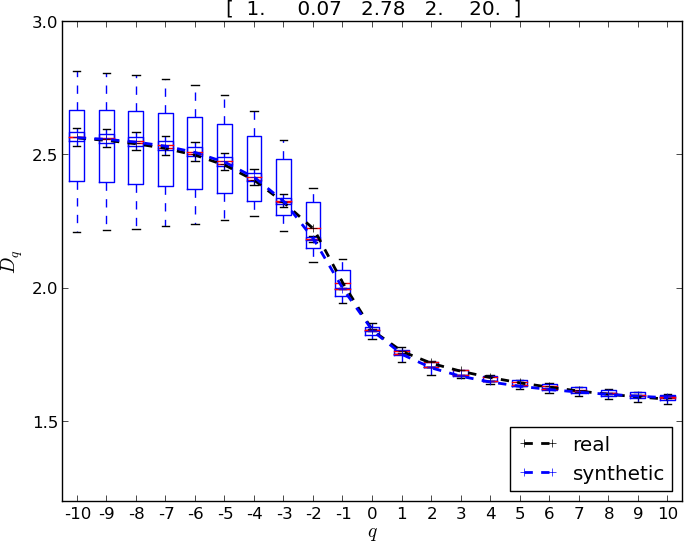
\includegraphics[width=9cm]{figures/bestboxplot}}
\caption[Mejores parámetros de síntesis para el tipo de pan {\em baguette}]{Mejores parámetros de síntesis para el tipo de pan {\em baguette}. El error total en medianas es de $\sim 0.21$.}
\label{bestboxplot}
\end{figure}

\begin{figure}[!ht]
\begin{center}
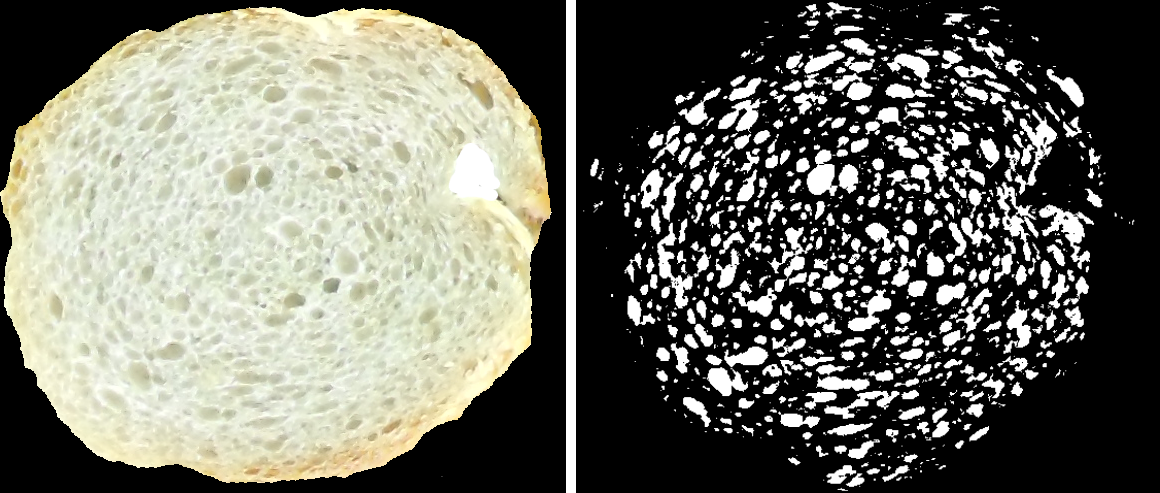
\includegraphics[width=13cm]{figures/realbin}
\caption{ Pan {\em baguette} real y ejemplo de binarización.}
\label{realbin}
\end{center}
\end{figure}

\begin{figure}[!ht]
\begin{center}
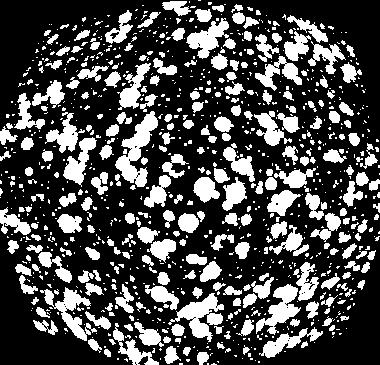
\includegraphics[width=6cm]{figures/best}
\caption{Resultado sintético mostrando características multifractales similares a imágenes reales del tipo de pan {\em baguette}.}
\label{best}
\end{center}
\end{figure}

Similarmente, encontramos parámetros para un tipo de pan casero utilizando la misma búsqueda:

\begin{align*}
k &= 0.69 \frac{N^{3}}{20} ,\\
d &=5.6,\\
r_{min} &=1,\\
r_{max} &=24.\\
paso &=1,
\end{align*}

La Fig.~\ref{bestboxplot2} muestra boxplots de panes reales y sintéticos de este tipo casero.
La Fig.~\ref{realbin2} y  Fig.~\ref{best2} muestran un ejemplo de binarizaciones de estas imágenes. 


\begin{figure}[!ht]
\centerline{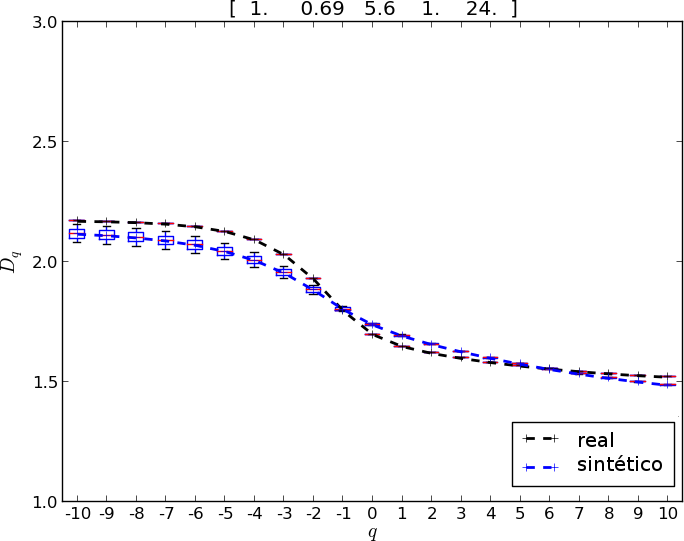
\includegraphics[width=9cm]{figures/bestboxplot2}}
\caption[Mejores parámetros de síntesis para un tipo casero de pan]{Mejores parámetros de síntesis para un tipo casero de pan. El error total en medianas es de $\sim 0.88$.}
\label{bestboxplot2}
\end{figure}

\begin{figure}[!ht]
\begin{center}
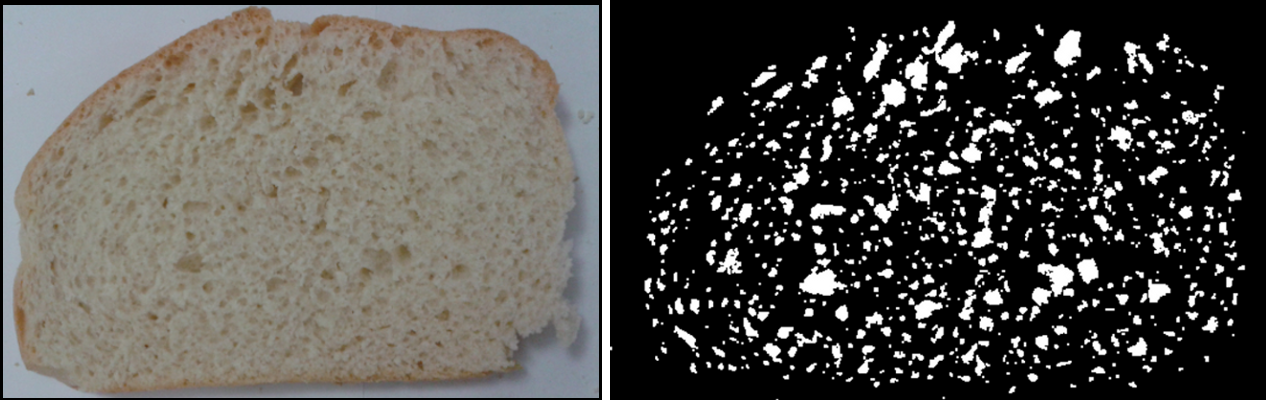
\includegraphics[width=13cm]{figures/realbin2}
\caption{ Pan casero real y ejemplo de binarización.}
\label{realbin2}
\end{center}
\end{figure}

\begin{figure}[!ht]
\begin{center}
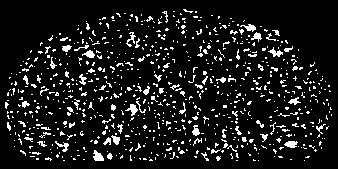
\includegraphics[width=8cm]{figures/best2}
\caption{Ejemplo de pan sintético con características similares a imágenes de un pan casero.}
\label{best2}
\end{center}
\end{figure}

%\section{Validación utilizando técnicas de Aprendizaje Profundo}

\section{Discusión y Conclusiones}

En este capítulo demostramos que los métodos fractales y sobre todo, multifractales, permiten capturar características útiles de panes, las cuales pueden utilizarse para caracterizarlos y clasificarlos.
Además, la información capturada resulta lo suficientemente descriptiva para utilizarse en la definición de parámetros de entrada a un algoritmo que genera versiones sintéticas de los mismos, las cuales fueron también validadas.
La apariencia de diferentes tipos de panes puede ser caracterizada exitosamente computando dimensiones multifractales de sus imágenes digitales.
Las DFs obtenidas por el método MFS cuyo $\alpha \in [0: 0.23]$ proveen una buena medida de la porosidad de la miga del pan, ya que mientras mayor la DF, mayor la porosidad.
Además, las DFs cuyo $\alpha \in [0.79: 1]$ permiten caracterizar la granularidad y la heterogeneidad en la distribución de sus burbujas.
El MFS contiene datos útiles para caracterizar las tres medidas, combinando la información en un único vector de características.

La utilización de características multifractales en la clasificación de dichas imágenes mostró además un excelente rendimiento.
El MFS demostró ser lo suficientemente preciso para realizar una clasificación de distintos tipos de panes y separar panes de otros objetos.
Los resultados superan otras características del estado del arte utilizadas en la literatura de visión por computador.
La información presente en los canales $L$, $a$ y $b$ del MFS de las imágenes transformadas al espacio de color CIELab obtuvieron los resultados más altos en la clasificación.
Este resultado parece ser consecuencia del comportamiento del espacio mencionado cuando existe más de un dispositivo de captura.
Se mostró además que el MFS resulta sensible a cambios en la iluminación durante la adquisición de las imágenes.

Por otro lado, el método multifractal Sandbox permite definir parámetros con la intención de aproximar la geometría de cualquier miga de pan, extrayendo parámetros para simular de manera precisa un tipo dado.
Las distribuciones de burbujas de nuestro modelo pueden adecuarse de manera estadística con algún tipo de pan deseado, gracias al análisis multifractal Sandbox.
Para comprobar esta afirmación, se realizaron pruebas con dos tipos de panes diferentes: {\em baguette} y un tipo de pan casero.
El espectro multifractal del pan casero resultó más dificultoso de sintetizar (es decir, los errores fueron mayores que aquellos del tipo {\em baguette}), pero a pesar de esto, las imágenes obtenidas resultan más que adecuadas para emular el tipo de pan deseado en computación gráfica.
El espectro multifractal presentó mayor dispersión en las dimensiones negativas ($q < 0$), 
lo cual significa que debido al límite de resolución en las imágenes, la distribución estadística resulta más difícil de capturar en escalas más pequeñas.

En este capítulo se demostró que la geometría macroscópica de la miga del pan puede ser fielmente aproximada por medio del algoritmo procedimental, el cual simula el proceso de fabricación del pan, presentado en el capítulo de modelado.
Los resultados presentados en este capítulo fueron publicados en congresos locales, una revista nacional y una revista internacional \cite{Baravalle2012, Baravalle2012_2, Baravalle2012_3, Baravalle2015}.


